\chapter{The A* Search Framework for MLP Training}
\label{chap:astar_framework}

The primary objective of this project is to reformulate the optimization challenge of training a Multilayer Perceptron (MLP) as a \textbf{shortest-path problem} within a discrete, high-dimensional weight space. This chapter introduces the framework designed to achieve this, detailing how the continuous weight space is discretized, how the nodes and edges of the search graph are defined, how the challenge of main memory saturation is managed and how the A* algorithm's is adapted to guide the network towards optimal weights.

\section{Discretization of the Weight Space}

The A* algorithm fundamentally operates on a discrete graph. Therefore, the continuous domain of real-valued weight parameters must be converted into a finite, discrete set of possible states. This is handled by the \texttt{QuantizedMLP} class.

\subsection{Quantized State Definition}
To define the search nodes, the floating-point parameters (weights and biases) of the MLP are subjected to uniform quantization. Given a predefined \textbf{quantization factor} ($Q$), every weight $w_i$ is rounded to the nearest multiple of $1/Q$.

$$w_{i, \text{quantized}} = \text{round}(w_i \cdot Q) / Q$$

The number of potential discrete weight configurations defines the size of the search space. To manage the complexity and avoid instability, the parameters are constrained to a defined numerical range $[\text{min\_range}, \text{max\_range}]$.

The total number of possible states is: 
$$[\text{Q} (\text{min\_range} + \text{max\_range}) + 1]^{N_{\text{params}}}$$

\subsection{State Representation and Hashing}
In the A* implementation, the efficacy of the algorithm relies on quickly checking if a particular weight configuration has been visited before, or if a better path to that configuration has been found. This requires a unique, hashable identifier for each state.

The \texttt{QuantizedMLP} utilizes the \texttt{get\_state\_hash()} method, which concatenates all quantized parameters into a single, ordered tuple of integers (by multiplying the quantized weights by the quantization factor $Q$). This tuple serves as the key in the Closed Set (represented by the \texttt{g\_costs} dictionary in the implementation) for tracking the minimum cost found so far to reach that state.

%====================================================================================================================================================================================================

\section{The Search Node}

In the context of A* based optimization, a search node $n$ is defined as a discrete point within a high-dimensional graph $\mathcal{G} = (\mathcal{V}, \mathcal{E})$. Each vertex $v \in \mathcal{V}$ represents a unique, quantized configuration of the neural network's weights and biases. The edges $\mathcal{E}$ are induced by the possible transitions permitted, which move the network from one quantized state to another.

A single search node $n$ is encapsulated by the \texttt{SearchNode} class, which maintains the following state and metadata:

\begin{enumerate}
    \item \textbf{Quantized State:} The current \texttt{QuantizedMLP} configuration, representing a unique coordinate in the quantized parameter space.
    \item \textbf{Cost-to-come ($g(n)$):} The cumulative cost incurred from the initial configuration to the current node, calculated as the sum of loss differentials along the path.
    \item \textbf{Heuristic Estimate ($h(n)$):} The estimate of the remaining cost to reach the target loss (the "goal"), here defined by the current loss value $L(n)$.
    \item \textbf{Total Estimated Cost ($f(n)$):} The evaluation function $f(n) = g(n) + h(n)$, which the A* algorithm uses to prioritize node exploration in the Open List.
    \item \textbf{Parent Pointer:} A reference to the preceding node in the search graph, allowing for the reconstruction of the optimal training trajectory upon convergence.
\end{enumerate}

%=============================================================================================================================================================================================================

\section{Defining Transitions: Neighborhood Generation Strategies}

The edges of the search graph are defined by the allowed transitions between weight configurations, generated by the \texttt{get\_neighbors} function. We implement a versatile framework supporting three distinct strategies for neighbor generation, each offering a different trade-off between structured and stochastic exploration.

In all methods, a neighbor state $s$ is generated from the current state $n$ by selecting a subset of parameters $\theta \in \text{Layer}_{\ell}$ and applying a discrete quantization step:
$$ \theta_{s} = \theta_{n} \pm \frac{1}{Q} \quad \forall \theta \in \text{Subset} $$

\subsection{Strategy 1: Single-Kernel Method}
This approach utilizes a unique set of kernel ($H \times W$ for weights, $L \times 1$ for biases) and stride ($x_s, y_s$) pairs applied consistently across all layers. The algorithm dynamically handles architectural constraints through \textbf{dynamic shrinking} (adaptive kernel scaling): if the target tensor dimensions are smaller than the defined kernel, the window is automatically clipped to fit the available parameter space. This ensures a consistent transition logic while maintaining robustness across heterogeneous layer sizes.

\subsection{Strategy 2: Layer-Wise Kernel Method}
To allow for higher degrees of freedom, this method supports per-layer customization, while retaining the \textbf{adaptive kernel scaling} mechanism to ensure compatibility with varying tensor dimensions. For each layer $\ell$, a specific weight kernel, bias kernel, and stride pair ($x_s, y_s$) are defined. This enables the search to adapt its "spatial reach" to the specific role of the layer. For instance, wider kernels may be utilized for initial layers to capture broad features, while narrower kernels can be used for final layers to perform fine-grained adjustments.

\begin{center}
\begin{figure}[H]
    \centering
    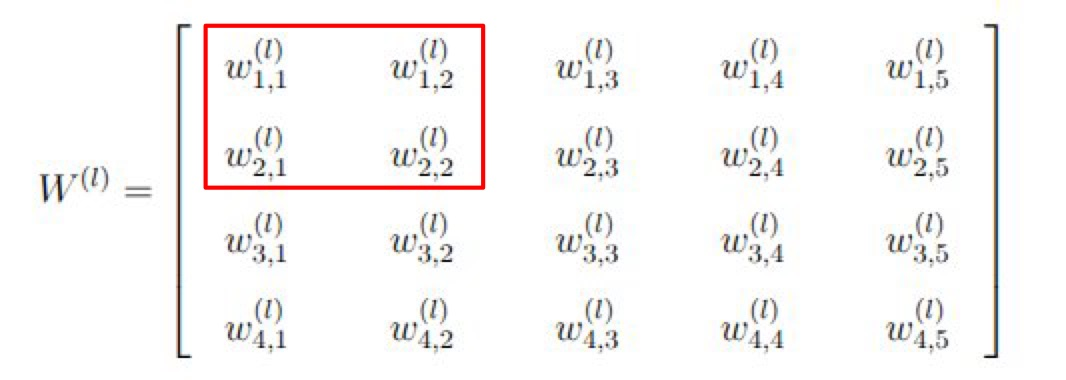
\includegraphics[width=0.7\textwidth]{figures/layer/matrix_1.jpg}
    \caption{Visualization of a $2 \times 2$ kernel at position (1,1) in a quantized weight matrix.}
\end{figure}
\end{center}

\begin{center}
\begin{figure}[H]
    \centering
    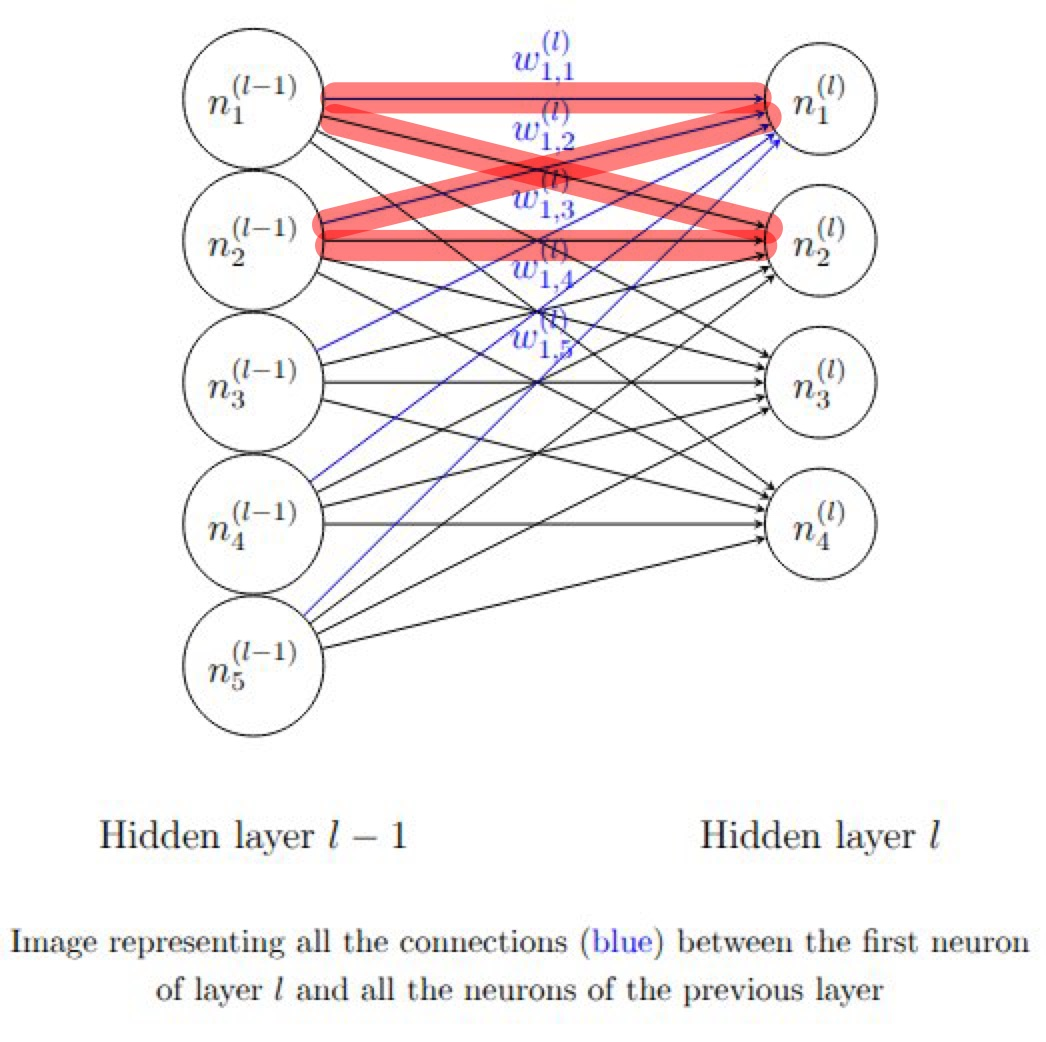
\includegraphics[width=0.7\textwidth]{figures/layer/layer_1.jpg}
    \caption{Connections within the MLP architecture specifically affected by a localized kernel update.}
\end{figure}
\end{center}

For both kernel-based strategies, the number of possible transitions (slides) per layer is determined by the valid window positions in an $M \times N$ matrix:
$$ \text{Slides}_{\ell} = \left( \lfloor \frac{M - H}{y_s} \rfloor + 1 \right) \times \left( \lfloor \frac{N - W}{x_s} \rfloor + 1 \right) $$


\subsection{Dynamic Kernel Reshaping}
\label{subsec:dynamic_kernel_reshaping}

To address the issue of convergence stagnation during the optimization process, we introduced a heuristic mechanism known as \textit{Dynamic Kernel Reshaping}. This technique is exclusively applied to the kernel-based neighbor generation strategies (\textit{Single-Kernel} and \textit{Layer-Wise Kernels}) and serves to adaptively refine the search granularity when the training loss hits a plateau.

\subsubsection{Plateau Detection Mechanism}
 The algorithm monitors the training trajectory to detect "stalling" conditions where the current kernel configuration fails to produce significant improvements.  This detection is governed by two hyperparameters:
\begin{itemize}
    \item \textbf{Loss Improvement Threshold ($\delta_{loss}$):} The minimum required decrement in training loss between two consecutive iterations ($L_t - L_{t+1}$) to be considered a valid improvement.
    \item \textbf{Dynamic Kernel Reshaping Patience ($P_{reshape}$):} A counter that tracks the number of consecutive iterations where the loss improvement has failed to meet $\delta_{loss}$.
\end{itemize}

\subsubsection{Dynamic Shrinking Process}
When the accumulated patience counter reaches the defined limit ($P_{reshape}$), the system infers that the search has reached a local optimum relative to the current coarse-grained kernel sizes. To facilitate finer exploration, a \textbf{shrinking event} is triggered.

During this event, the dimensions of the kernels ($K$) and strides ($S$) are reduced by fixed decrement values:
$$ K_{new} = \max(K_{min}, K_{old} - \Delta_k) $$
$$ S_{new} = \max(S_{min}, S_{old} - \Delta_s) $$

where $\Delta_k$ and $\Delta_s$ represent the \textit{kernel decrement} and \textit{stride decrement} parameters (defaulting to 1), and $K_{min}, S_{min}$ represent the minimum allowed shapes to ensure structural validity.

This process allows the $A^*$ search to transition from a broad, global exploration phase to a high-resolution local refinement phase. The reshaping mechanism remains active throughout the training lifecycle; if the patience is exhausted again at the new resolution, the kernels are shrunk further until they reach their minimum bounds or the training completes the maximum allocated iterations.


\subsection{Adaptive Kernel Scaling}
In scenarios where the target network architecture contains layers with parameter tensors smaller than the predefined kernel dimensions, an \textbf{adaptive kernel scaling strategy} is employed. This mechanism allows scaling the kernel size ($K$) and strides ($S$) to fit the specific geometry of the parent tensor.

\subsubsection{2D Weight Matrices}
For a weight matrix of shape $(M, N)$, let the initial weight kernel shape be defined as $\mathbf{k}_w = [k_y, k_x]$. If the matrix dimensions are smaller than the kernel size in any axis ($M < k_y$ or $N < k_x$), the updated kernel $\mathbf{k}'_w = [k'_y, k'_x]$ and strides $s'_x, s'_y$ are calculated as follows:

First, we clip the kernel to the maximum available dimensions:
$$ k'_{y, \text{clip}} = \min(M, k_y), \quad k'_{x, \text{clip}} = \min(N, k_x) $$

To maintain a search granularity that is finer than the layer itself, we identify the smaller of these dimensions and reduce it by half:
$$ \text{index}_{\min} = \text{argmin}(k'_{y, \text{clip}}, k'_{x, \text{clip}}) $$
$$ k'_{\text{index}_{\min}} = \max\left(1, \lfloor k'_{\text{index}_{\min}, \text{clip}} / 2 \rfloor\right) $$

Finally, the traversal strides are set equal to the new kernel dimensions to ensure full, non-overlapping coverage of the search space:
$$ s'_x = k'_x, \quad s'_y = k'_y $$

\subsubsection{1D Bias Vectors}
For bias vectors of length $L$, the 1D kernel $k_b$ is adjusted if $L < k_b$. The new kernel $k'_b$ and stride $s'_y$ are defined by:
$$ k'_b = \max\left(1, \lfloor \min(L, k_b) / 2 \rfloor\right) $$
$$ s'_y = k'_b $$

This adaptation ensures that even for extremely small layers (such as the final output layer of a regressor), the branching factor remains bounded and the search can still identify discrete updates without requiring manual hyperparameter reconfiguration per layer.

\subsection{Strategy 3: Random Sampling Method}
This strategy employs a stochastic approach to define the target set of parameters, governed by two key hyperparameters:
\begin{itemize}
    \item \textbf{Perturbation Ratio ($r_p$):} Determines the percentage of total parameters within a layer modified in a single transition. For a layer with $N_{\text{total}}$ parameters, each neighbor modifies $\lceil r_p \cdot N_{\text{total}} \rceil$ weights selected via random sampling.
    \item \textbf{Search Coverage Ratio ($r_c$):} Determines the total number of unique neighbors generated for each layer, calculated as $\lceil r_c \cdot N_{\text{total}} \rceil$.
\end{itemize}





\subsection{Dynamic Quantization}
\label{subsec:dynamic_quantization}

While Dynamic Kernel Reshaping addresses the \textit{spatial} resolution of the search (i.e., how many parameters are changed), \textbf{Dynamic Quantization} addresses the \textit{numerical} resolution of the updates (i.e., how much the parameters change). Unlike kernel reshaping, this technique is universally applicable to all three neighbor generation strategies.

\subsubsection{Stagnation and Trigger Logic}
Similar to the reshaping mechanism, this strategy employs a heuristic based on training stagnation. The algorithm monitors the loss trajectory using the global \textit{Loss Improvement Threshold}. A dedicated counter, the \textbf{Dynamic Quantization Patience}, tracks the number of consecutive iterations where the training loss fails to improve beyond this threshold.

\subsubsection{Quantization Refinement}
When the patience counter is exhausted, it indicates that the current discretization of the weight space is too coarse to identify a valid descent direction effectively, the "grid" of allowable weight values is straddling the local minimum without landing in it.

To resolve this, the quantization factor $Q$ is \textbf{increased}. Since the discrete step size for any parameter update is defined as $\Delta \theta = \pm \frac{1}{Q}$, increasing $Q$ results in a smaller, more precise step size:
$$ Q_{new} = Q_{old} * \Delta_Q \quad \implies \quad \frac{1}{Q_{new}} < \frac{1}{Q_{old}} $$

where $\Delta_Q$ represents the \textit{Quantization Factor Multiplier} (defaulted to 10).

\subsubsection{Operational Impact}
By dynamically increasing the quantization factor, the search space transitions from a coarse grid to a fine-grained mesh. This allows the algorithm to perform high-precision "micro-updates," enabling the network to settle into deeper minima that were previously inaccessible due to the rigidity of the initial discrete steps. This process can repeat iteratively, progressively refining the numerical precision until the training concludes.





\subsection{Mathematical Comparison of Branching Factors}
The branching factor $B$ represents the number of successor nodes generated from a single parent node. A comparison of the branching factors between the Layer-wise Kernel and Random Sampling methods highlights the difference in search space density:

\begin{enumerate}
    \item \textbf{Kernel-Wise Branching ($B_K$):} The branching factor is strictly determined by the geometry of the layers and the chosen kernels and strides:
    $$ B_K = 2 \cdot \sum_{\ell \in \text{Layers}} \left( \text{Slides}_{\text{weights}, \ell} + \text{Slides}_{\text{biases}, \ell} \right) $$
    
    \item \textbf{Random Sampling Branching ($B_R$):} The branching factor is proportional to the total parameter count $N$ of the network:
    $$ B_R = 2 \cdot \sum_{\ell \in \text{Layers}} \lceil r_c \cdot N_{\ell} \rceil $$
\end{enumerate}

\subsection{Comparative Analysis: Structured vs. Stochastic Exploration}

The three proposed neighborhood generation strategies represent different philosophies in exploring the high-dimensional quantized parameter space. Their effectiveness is evaluated based on four primary criteria: spatial locality, search space pruning, exploration capacity, and hyperparameter complexity.

\begin{itemize}
    \item \textbf{Single-Kernel Method}
    \begin{itemize}
        \item \textbf{Pros:} Provides extreme \textit{search space pruning} by enforcing a uniform transition rule across the entire network. It maximizes \textit{spatial locality} by ensuring that every weight update is part of a cohesive geometric block.
        \item \textbf{Cons:} Limited \textit{exploration} flexibility; if the network has layers of vastly different sizes (e.g., a massive hidden layer followed by a tiny output layer), the fixed kernel size may be too coarse for some layers and too fine for others.
    \end{itemize}

    \item \textbf{Layer-Wise Kernel Method}
    \begin{itemize}
        \item \textbf{Pros:} Provides an enhanced degree of architectural flexibility while maintaining the inherent advantages of \textit{spatial locality} through localized weight updates. By tailoring kernel sizes and strides to the specific dimensions of each layer, it optimizes the \textit{search space pruning} for the architecture's specific geometry. This prevents "blind spots" in smaller layers while maintaining high-speed traversal in larger ones.
        \item \textbf{Cons:} Increases the hyperparameter search space. Determining the optimal $(WK, BK, S)$ triplet for every layer adds significant complexity to the pre-training experimental setup.
    \end{itemize}

    \item \textbf{Random Sampling Method}
    \begin{itemize}
        \item \textbf{Pros:} Superior \textit{exploration} capacity. By breaking the constraint of geometric locality, it can discover non-obvious weight correlations and escape local minima where kernel-based movements might stall. It allows for a dense or sparse search controlled entirely by the \textit{perturbation ratio} and \textit{search coverage ratio} parameters.
        \item \textbf{Cons:} No \textit{spatial locality} is assumed and because updates are stochastic, the search can become "noisy," leading to lower efficiency as the algorithm may explore many disjoint directions that do not contribute to a cohesive functional change in the network's output.
    \end{itemize}
\end{itemize}

\begin{table}[H]
\centering
\caption{Comparison of Neighbor Generation Strategies}
\label{tab:strategy_comparison}
\begin{tabular}{lcccc}
\hline
\textbf{Feature} & \textbf{Single Kernel} & \textbf{Layer-Wise} & \textbf{Random} \\ \hline
Locality Preservation & High & High & None \\
Search Space Pruning & High & Moderate & Variable \\
Exploration Breadth & Low & Moderate & High \\
Hyperparameter Complexity & Low & High & Low \\ \hline
\end{tabular}
\end{table}

%=============================================================================================================================================================================================================

\section{Memory Optimization: Beam Search Integration}

A significant challenge in applying the A* search algorithm to neural network optimization is the memory-intensive nature of maintaining the \textit{Open} and \textit{Closed} sets. In large-scale architectures, the branching factor $B$ scales with the total number of parameters, leading to an exponential growth of the search tree. Empirical observations showed that without optimization, the search often encountered premature termination due to system RAM saturation. This phenomenon, in some MLP architectures tested, prevented the algorithm from surpassing 100--200 iterations, leaving the network in a sub-optimal state despite remaining potential for loss reduction.

To mitigate this bottleneck, a \textbf{Beam Search memory optimization} was designed and integrated into the search framework. This technique effectively caps the memory footprint by limiting the maximum size of the search frontier.

\subsection{Periodic Set Pruning and Memory Regulation}
The optimization is governed by the \textit{Beam Width} ($BW$) parameter, which defines the target maximum capacity for the \textit{Open} and \textit{Closed} sets. In this implementation, memory regulation is applied periodically rather than at every discrete time step; in our experimental benchmark, this check occurs every 50 iterations.

Consequently, the dimensions of the search sets are not strictly fixed at every step. Between two pruning cycles, the sets are allowed to grow dynamically to accommodate the branching factor of the network. Once the iteration threshold is reached, the algorithm evaluates the current size of the sets. If they exceed the defined limit, a pruning operation is triggered to restore the memory footprint to the specified $BW$:

\begin{enumerate}
    \item \textbf{Ranking:} All nodes currently in the set are sorted according to their evaluation function $f(n) = g(n) + h(n)$.
    \item \textbf{Truncation:} Only the top $BW$ nodes, those representing the most promising search trajectories, are retained.
    \item \textbf{Memory Release:} All remaining nodes are purged from the main memory, effectively resetting the search frontier to a manageable scale.
\end{enumerate}

This "pulsed" pruning approach strikes a balance between allowing the search to explore diverse local branches in the short term and maintaining long-term stability in the face of hardware memory constraints.

\subsection{Impact on Training Longevity}
The implementation of the Beam Search optimization has demonstrated a profound impact on the scalability of the training process, particularly in deeper architectures. By enforcing a fixed memory bound, the algorithm can navigate the parameter space for significantly longer durations. 

\begin{itemize}
    \item \textbf{Scalability:} Networks that previously exhausted memory within 200 iterations can now reliably reach fixed thresholds of $2,000$ iterations or more.
    \item \textbf{Loss Minimization:} The ability to sustain longer search trajectories allows the A* algorithm to escape local plateaus and locate deeper minima in the loss landscape that were previously unreachable due to hardware constraints.
    \item \textbf{Tuning:} The $BW$ parameter acts as a trade-off between search completeness and memory safety. A higher $BW$ allows for a more exhaustive search closer to the original A*, while a lower $BW$ ensures stability in environments with limited hardware resources.
\end{itemize}

This optimization transforms the A* approach from a memory-bounded search into a scalable iterative optimizer, making it viable for architectures that would otherwise be computationally prohibitive.

%=============================================================================================================================================================================================================

\section{The A* Training Loop Implementation}

The core training logic is contained within the \texttt{Trainer} class, which manages the A* search:
\begin{enumerate}
    \item \textbf{Initialization:} The process begins by creating an \texttt{initial\_node} from the starting MLP weights. This node is placed in the priority queue (\texttt{open\_set}).
    \item \textbf{Iteration:} In each iteration, the node with the lowest $f(n)$ is retrieved from the \texttt{open\_set}.
    \item \textbf{Optimality Check:} Before expanding the node, the current path cost $g(n)$ is checked against the minimum cost previously recorded for that state in \texttt{g\_costs} to ensure that A* always processes the optimal path to a given state first.
    \item \textbf{Expansion:} Neighbors are generated by the transition rule ($\pm 1/Q$ change to a weight subset).
    \item \textbf{Cost Update:} For each neighbor, the new $g$ and $h$ values are calculated. If the new path to the neighbor results in a lower cost-to-come ($g_{\text{new}} < g_{\text{old}}$), the neighbor is either updated in the search space or added to the \texttt{open\_set}.
    \item \textbf{Termination:} The search terminates when either the best node retrieved from the \texttt{open\_set} satisfies the goal condition ($h(n) = 0$) or the maximum number of iterations is reached.
\end{enumerate}

%=============================================================================================================================================================================================================



